
%(BEGIN_QUESTION)
% Copyright 2007, Tony R. Kuphaldt, released under the Creative Commons Attribution License (v 1.0)
% This means you may do almost anything with this work of mine, so long as you give me proper credit

Examine this process trend, showing the response of the process variable to a 10\% up-and-down step change in the controller output (placed in manual mode):

$$\includegraphics[width=15.5cm]{i01718x01.eps}$$

What characteristics of the process (and its related instrumentation) can you discern from this trend?  Based on this information, do you think the process might benefit from a controller with aggressive P, I, or D action?  Explain why or why not for each action.

\vskip 10pt

A very common misconception among students first learning how to analyze loop trend graphs is to mistakenly interpret the above trend as indication that the controller already has proportional action programmed into it.  Explain why this is a misconception, and how we can avoid it.

\vskip 20pt \vbox{\hrule \hbox{\strut \vrule{} {\bf Suggestions for Socratic discussion} \vrule} \hrule}

\begin{itemize}
\item{} One area of confusion for new students is whether any given trend graph reveals an {\it open-loop} test or a {\it closed-loop} test.  Explain how it is possible to discern the kind of test done on this process just by looking at the trend lines.
\item{} Explain why it is important to determine whether the trend graph reveals an {\it open-loop} test or a {\it closed-loop} test.  What difference does this determination make?
\item{} Based on what you see here, does the controller need to be configured for {\it direct} action or for {\it reverse} action?
\end{itemize}

\underbar{file i01718}
%(END_QUESTION)





%(BEGIN_ANSWER)

This is definitely a self-regulating process with an overall process gain (including instruments) of about 2.  The fact that it is self-regulating suggests it may be primarily controlled by integral action.  The fact that it is relatively fast-acting suggests it may tolerate rather aggressive integral action.  This same fact suggests derivative action would {\it not} do much good.

\vskip 10pt

The reason new students commit the error of interpreting a trend such as this as an indication of {\it controller} proportional action is because they do not recognize the significance of the controller being in manual mode rather than automatic mode.  In manual mode as we see here (revealed as such by the long, flat periods of the output signal despite changes in PV), what the trend reveals to us are the characteristics of the {\it process} itself, not of the {\it controller}.  What students are accustomed to seeing is a matched-shape response between PV and output being indicative of proportional action {\it in a controller that is in automatic mode, actively trying to control a process}.  Here, where any automatic control action has been disabled, the response of the PV to any change in output is revealing to us how the process actually responds to the valve.  Thus, a trend where PV steps up in a manner similar to the output step-change, we know that the {\it process} has a self-regulating characteristic, but we don't know anything yet about how the controller happens to be set up for automatic mode.

%(END_ANSWER)





%(BEGIN_NOTES)

More subtle, but definitely evident here, is a slight amount of hysteresis in the control valve and/or the measuring instrument.  Note how the PV does not return precisely to the value it began when the output is returned back to 35\%.  It should be noted, however, that this difference in PV may be due to a process load change that happened while the controller output was at 45\%.


%INDEX% Control, PID tuning: predicting PID requirements based on open-loop response

%(END_NOTES)


